Прогресс в области машинного обучения и разработки интеллектуальных ассистентов ведет к росту потребности в высококачественных корпусах текстов и аннотированных изображений.
 Наиболее остро проявляется недостаток систематизированных методических материалов на русском языке. 


\textit{Определение} \textbf{Оптическое распознавание символов} (OCR) представляет собой процесс автоматического преобразования текста,
 представленного в виде изображения или сканированного документа, в текстовый формат.
 
Первоначально изображение документа подвергается предварительной обработке, такой как удаление шума или коррекция искажений. 
Затем происходит сегментация изображения, то есть разделение его на отдельные символы или группы символов.

Далее, при помощи алгоритмов распознавания, включающих методы машинного обучения и компьютерного зрения, 
символы на изображении анализируются и сопоставляются с соответствующими символами из набора знаков. Этот этап включает в себя распознавание формы символов, их контекста и других характеристик, что позволяет определить, какие символы были изображены на сканированном документе.

В завершение, распознанные символы объединяются в слова, предложения и абзацы, формируя полноценный текстовый документ. Точность и эффективность процесса OCR зависят от качества изображения, используемых алгоритмов распознавания, а также от языка и структуры текста. В современных приложениях OCR широко используются в различных областях, включая сканирование документов, распознавание номеров автомобильных номеров, оптическое чтение рукописных текстов и другие приложения, где требуется автоматическое извлечение текста из изображений.

Существует множество пакетов для выполнения OCR \begin{itemize}
    \item Nougat  \cite{blecher2023nougat}
    \item \cite{smith2007overview}
    \item LayoutParser \cite{shen2021layoutparser}
\end{itemize}

К сожалению, доступные открытые решения либо не поддерживают русский язык, либо не предназначены для работы с формулами.
Для решения автора был разработан открытый программный пакет для Python ShuemacherOCR
, предназначенный для масштабного анализа русской естественно-научной методической литературы.
В состав пакета входят модули как для обработки отдельных изображений, 
так и полноценных документов, позволяющие, извлекать данные в структурированном виде. 
Для решения задачи пакет использует нейросетевые алгоритмы. 
Ключевой особенностью пакета  является возможность выделять в тексте на русском языке строчные математические формулы.
Установка выполняется из открытого реестра пакетов PyPI с помощью менеджера pip или
из репозитория \footnote{\url{https://github.com/NMashalov/SchumacherOCR}}. 

Данные задач были собраны из открытых педагогических источников \cite{libmipt}\cite{mathedu} 
c обязательным указанием при публикации ссылок на источники.

Распознание текста по изображению выполняется нейросетью архитектуры Nougat \cite{blecher2023nougat}.
Особенностью данной архитектуры является быстрая адаптация под новые виды данных и работа с целым изображением, 
без необходимости промежуточного поиска регионов с текстом. 

Обучение сети проводилось на корпусе препринтов статей  \cite{clement2019use},
переведенных на русский язык с помощью интеллектуального ассистента ChatGPT \cite{ouyang2022training}. 
Выбор был связан с возможностью сохранять оригинальную разметку TeX-документов. 

Для валидации результатов был разработан открытый датасет, 
позволяющий измерить качество распознавания \footnote{\url{https://huggingface.co/datasets/NMashalov/ru_educational_book_datasets}} .

Разметка для обучения проводилось с помощью обращения к сервису компании MathPix. Метрики качества  приведены в таблице 1 и сопоставимы с результатами оригинальной модели Nougat.

\begin{center}
    \begin{tabular}{||c c c||} 
     \hline
     \text{Параметр} & \text{Тренировочная выборка} & \text{Отложенная выборка} \\
     \hline\hline
     \text{BLEU} & 83.2 & 80.4  \\ 
     \hline
     \text{Edit distance} & 0.15 & 0.17 \\
     \hline
    \end{tabular}
\end{center}

Для обучения на полученных данных была использована нейронная сеть YOLO \cite{redmon2016you}. Эта архитектура нейронной сети имеет способность эффективно дообучаться на небольших выборках данных, что позволяет достигать удовлетворительных результатов.
Для ситуаций, где число аннотаций и число изображений на изображении не совпадало, применялся алгоритм на двудольном графе, направленный на максимизацию числа пар.
 
Для получения обучающей выборки была проведена разметка части датасета. Каждое изображение включает в себя текстовую информацию, а также различные чертежи и формулы, характерные для данной области знаний.

Процесс разметки включал создание аннотаций для каждого изображения, 
а именно выделение границ объектов, таких как текстовые блоки, формулы и чертежи. 
Этот процесс требовал точности и внимательности для корректного определения границ объектов на изображении и их соответствия с аннотациями.

Для расширения датасета и обеспечения его разнообразия была применена аугментация данных. 
Применялись повороты, масштабирование, изменение освещения и отражение, позволили создать дополнительные вариации входных данных. 
Это способствовало увеличению разнообразия обучающей выборки и повышению устойчивости модели к различным вариациям данных, что важно для обеспечения ее эффективности в реальных условиях различной разметки страницы.

\begin{figure}[h]
    \centering
    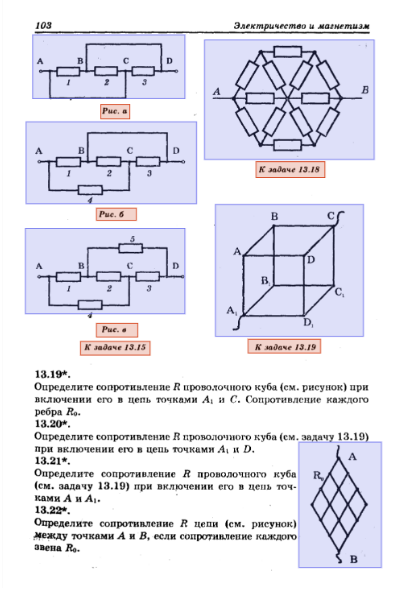
\includegraphics[width=0.5\textwidth]{assets/work/dataset/kirik_labeling.png}
    \caption{Пример аннотированной иллюстрации из книги Генденштейн, Кирик, Гельфгат: 1001 задача по физике}
    \label{annotation}
\end{figure}

Метрическая оценка результатов выделения иллюстрации и аннотации 

\begin{center}
    \begin{tabular}{||c c c||} 
     \hline
     \text{Параметр} & \text{Тренировочная выборка} & \text{Отложенная выборка} \\
     \hline\hline
     \text{mAp} & 78.4 & 75.4  \\ 
     \hline
     \text{Точность распознавания ребер  “изображение-аннотация”}  & 75.2 & 72.0 \\
     \hline
    \end{tabular}
\end{center}

\begin{figure}[h]
    \centering
    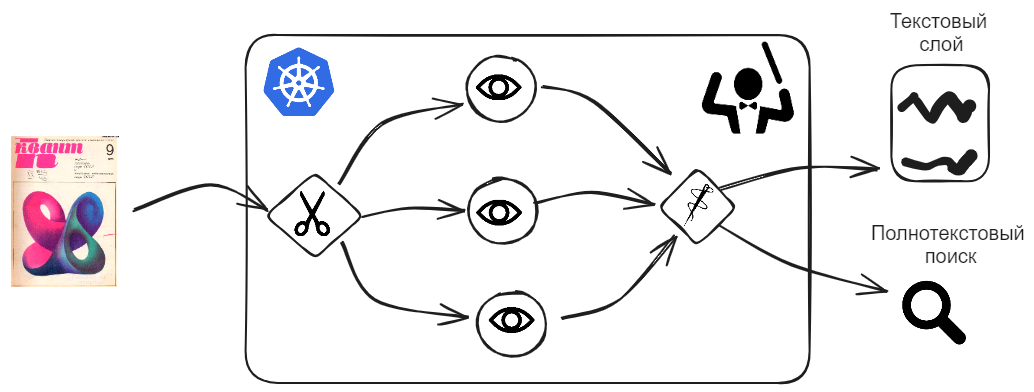
\includegraphics[width=0.5\textwidth]{assets/work/dataset/saga.excalidraw.png}
    \caption{Итоговая разметка выполняется посредством распределенных вычислений}
    \label{annotation}
\end{figure}







